\documentclass[onecolumn, draftclsnofoot,10pt, compsoc]{IEEEtran}
\hbadness=1000 % suppress warnings
\usepackage{graphicx}
\usepackage{url}
\usepackage{setspace}
\usepackage{hyperref}
\usepackage{listings}
\usepackage{cite}
\usepackage{geometry}

\geometry{textheight=9.5in, textwidth=7in}

% 1. Fill in these details
\def \CapstoneTeamName{		Aerolyzer}
\def \CapstoneTeamNumber{		19}
\def \GroupMemberOne{			Kin-Ho Lam}
\def \CapstoneProjectName{		Aerolyzer}
\def \CapstoneSponsorCompany{	NASA JPL}
\def \CapstoneSponsorPerson{		Kim Whitehall}


% 2. Uncomment the appropriate line below so that the document type works
\def \DocType{		%Problem Statement
	%Requirements Document
	%Technology Review
	%Design Document
	Progress Report
}

\newcommand{\NameSigPair}[1]{\par
	\makebox[2.75in][r]{#1} \hfil 	\makebox[3.25in]{\makebox[2.25in]{\hrulefill} \hfill		\makebox[.75in]{\hrulefill}}
	\par\vspace{-12pt} \textit{\tiny\noindent
		\makebox[2.75in]{} \hfil		\makebox[3.25in]{\makebox[2.25in][r]{Signature} \hfill	\makebox[.75in][r]{Date}}}}
% 3. If the document is not to be signed, uncomment the RENEWcommand below
\renewcommand{\NameSigPair}[1]{#1}

%%%%%%%%%%%%%%%%%%%%%%%%%%%%%%%%%%%%%%%
\graphicspath{{images/}}
\begin{document}
	\begin{titlepage}
		\pagenumbering{gobble}
		\begin{singlespace}
			
\includegraphics[height=4cm,natwidth=345,natheight=435]{images/coe_v_spot1.png}
			\hfill 
			% 4. If you have a logo, use this includegraphics command to put it on the coversheet.
			%\includegraphics[height=4cm]{CompanyLogo}   
			\par\vspace{.2in}
			\centering
			\scshape{
				\huge CS Capstone \DocType \par
				{\large\today}\par
				\vspace{.5in}
				\textbf{\Huge\CapstoneProjectName}\par
				\vfill
				{\large Prepared for}\par
				\Huge \CapstoneSponsorCompany\par
				\vspace{5pt}
				{\Large\NameSigPair{\CapstoneSponsorPerson}\par}
				{\large Prepared by }\par
				Group\CapstoneTeamNumber\par
				% 5. comment out the line below this one if you do not wish to name your team
				\CapstoneTeamName\par 
				\vspace{5pt}
				{\large
					\NameSigPair{\GroupMemberOne}\par
				}
				\vspace{20pt}
			}
			\begin{abstract}  
				The Aerolyzer Project aims to deliver a new source of air quality and weather information through leveraging existing weather data and image analysis algorithms.
				When complete, this open-source project shall feature a Python library that uses image classification and third-party weather APIs, displayed with an intuitive web-based user interface.
				This document outlines the software design descriptions for the Aerolyzer Library. 
			\end{abstract}     
		\end{singlespace}
	\end{titlepage}

\section{Table of Contents}
\tableofcontents
\bibliographystyle{IEEEtran}
\bibliography{ref}
\clearpage

\begin{singlespace}

	\section{Project Purpose}

	\section{Current State}

	\section{Issues}

	\section{Week-by-week summary}
		\subsection{Week 1}

		\subsection{Week 2}

		\subsection{Week 3}

		\subsection{Week 4}

		\subsection{Week 5}

		\subsection{Week 6}

		\subsection{Week 7}

		\subsection{Week 8}

		\subsection{Week 9}

		\subsection{Week 10}

	\section{Horizon Detection Filter}
      \subsection{Design Elements - OpenCV \& Google Tensorflow}
      		\subsubsection{Design Attributes}
          		Outlined in the Software Design Document, a horizon detection filter shall be created using OpenCV and other python libraries as required. OpenCV is a BSD-licensed computer-vision library with many relevant sub-modules. Containing over 2,500 algorithms, OpenCV can analyze images and videos, recognize faces, identify objects, perform visual transformations, and more. One can use image transformations to normalize image data such that a classifier can more easily distinguish what is in a given image. \cite{svm}

				An advanced machine learning library, Google Tensorflow can build versatile and accurate predictive data models provided a large dataset of training images. One can apply Tensorflow to the Aerolyzer project by training its inception module to recognize patterns in a large dataset consisting of acceptable images of the horizon. A human will need manually pre-classify and build a test dataset consisting of acceptable images. \ref{acc_img}  Tensorflow’s ease of use, proven library, and ample documentation makes it a potential candidate to create a powerful image classifier. \cite{rhnvrm} \cite{RNN}

				I have designed and tested two horizon detection classifiers using OpenCV 3.3.0. Ongoing work on the project can be viewed in the Aerolyzer library’s open-source Github. These classifiers are horizon detection by straight line and horizon detection by color threshold.

          \subsubsection{Design Relationships}
					.\\
					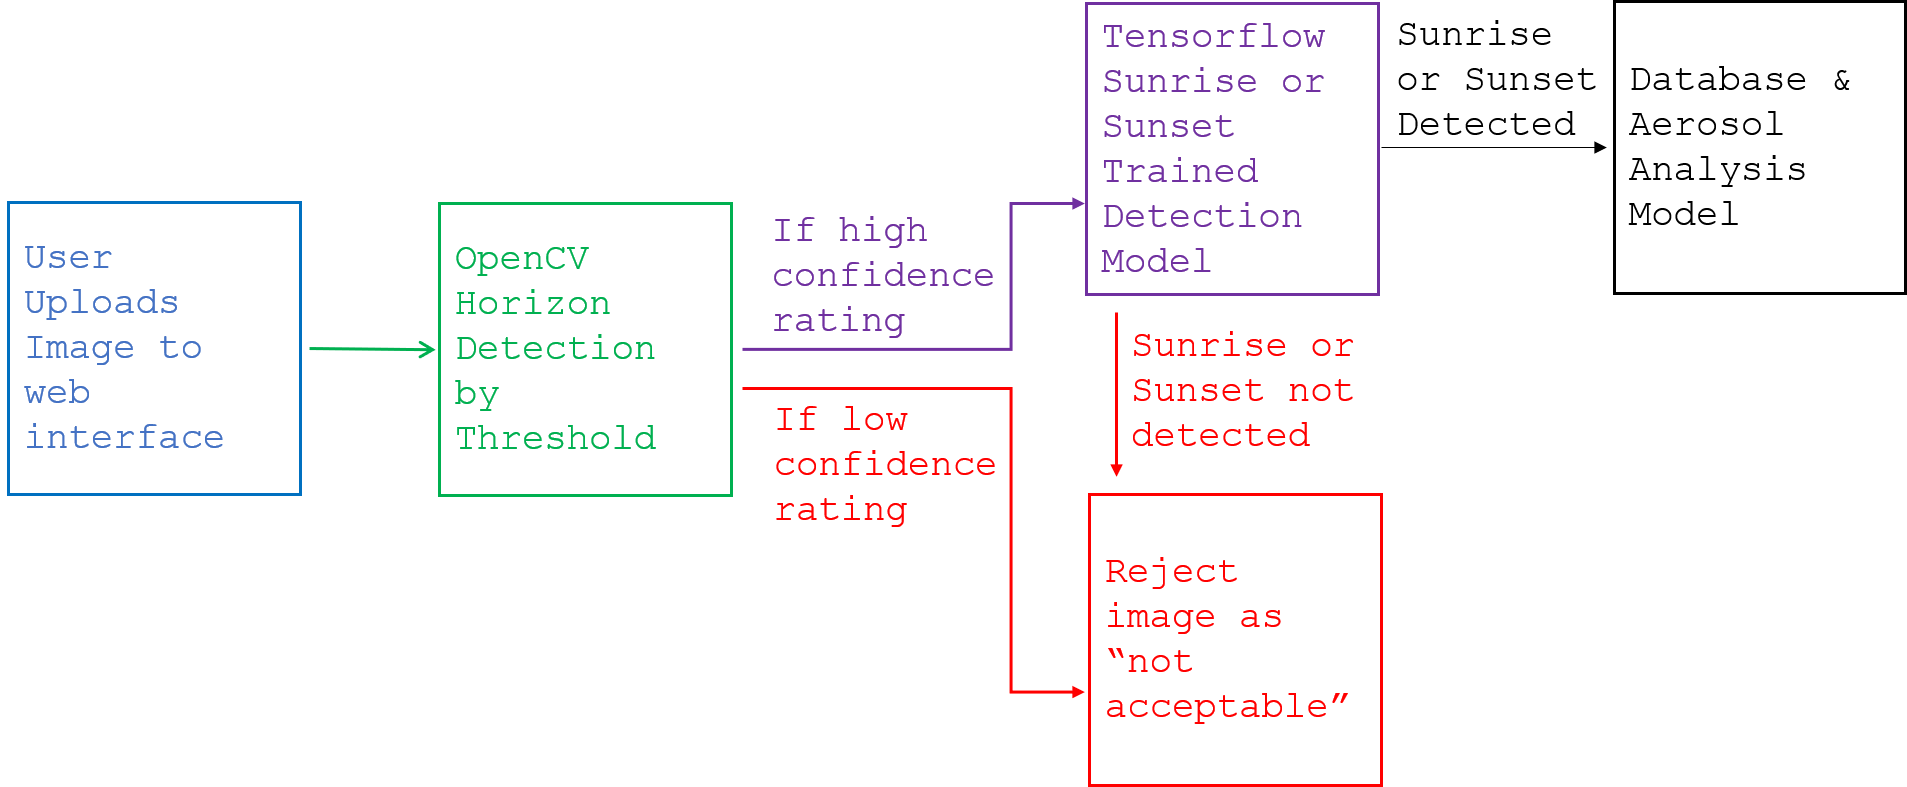
\includegraphics[width=4.5in,natwidth=1907,natheight=787]{images/tensor.png}

          \subsubsection{Design Constraints}
          		Aerolyzer’s unique image criterion necessitates a predictive data model capable of detecting horizons with a minimum of 66\% certainty and sunsets or sunrises with a minimum of 50\% certainty. Efficient and expedient algorithm performance is necessary due to the expected user base who will be waiting for Aerolyzer to service their request. Pending further research, these criterion are achievable through OpenCV and Tensorflow. More computer vision libraries or modules may be required.
      
      \subsubsection{Design overlays}
      		\subsubsection{OpenCV Horizon Detection by Straight Line Algorithm}
      			Horizon detection by straight line seeks to detect the simplest possible acceptable image; a picture of the sunset/sunrise without obstructions. In this case, one can expect the most visible longest and straightest line in an image to be the horizon. With this assumption, the Horizon Detection by Straight Line algorithm shall accept or reject an image through the following procedure:
      			\begin{enumerate}
      				\item Upon receiving an image, detect the longest and straightest line.
      				\item If there is no straight line stretching across the image, reject it.
      			\end{enumerate}
      			As a proof of concept, the algorithm is implemented in the following python function. This algorithm draws a straight green line where it believes the horizon is.
      			\lstinputlisting[language=Python,basicstyle=small]{code/HorizonDetectionbyStraightLine.py}
     			
     			Upon being fed an image, the Horizon Detection by Straight Line’s algorithm works as follows:
				

				\begin{enumerate}
					\item Perform a gaussian blur on the image
					\item Convert the image to grayscale
					\item Perform Canny Edge Detection \cite{svm}
					\item Perform Hough Line Transformation \cite{svm}
					\item If there is a straight line, draw a green line spanning across the image. This is the classified horizon.
					\item Else, if there are no straight lines, then reject the image.
				\end{enumerate}


				This approach works well for some images such as fig X pulled from the Aerolyzer test image album. However, it is clear that this approach does not work for all cases, as seen in fig Y, detecting the horizon by straight line fails in images with a complex foreground that contains many straight lines. A new algorithm is necessary to enhance detection accuracy.
				\\
				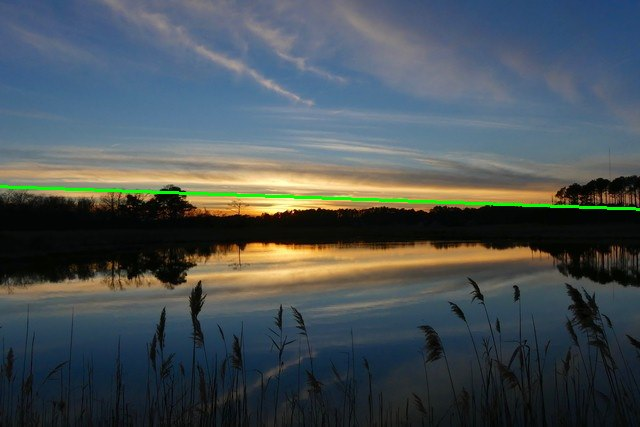
\includegraphics[width=4.5in,natwidth=640,natheight=427]{images/line1.jpg}
				\\
 				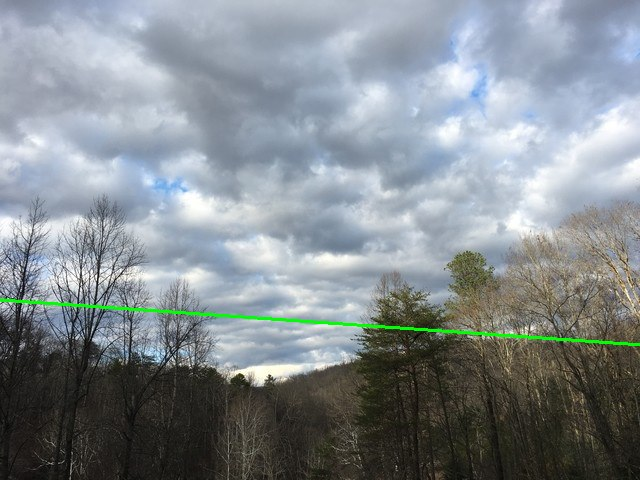
\includegraphics[width=4.5in,natwidth=640,natheight=480]{images/line2.jpg}

				\subsubsection{OpenCV Horizon Detection by Threshold}
					Horizon Detection by Threshold is a more versatile method compared to straight line detection because it relies on segmenting color distribution. Detection by Threshold was designed to classify images that contain complex foregrounds by distinguishing what part of the image is the sky. The Threshold algorithm shall accept or reject an image through the following procedure:
					\begin{enumerate}
						\item Separate the image by distinct color spaces
						\item Perform a binary threshold with the minimum color threshold being the color of the sky.
						\item Calculate the area of the largest continuous contour that is within the sky color threshold.
						\item Apply a statistical function to ratio the area of sky color over the total area of the image to produce a confidence rating. A high confidence rating shall indicate that the image contains a horizon while a low confidence rating indicates there is no horizon.
					\end{enumerate}

					As a proof of concept, the algorithm is implemented in the following python function. This algorithm draws a green outline of what it believes to be the sky.

					\lstinputlisting[language=Python]{code/HorizonDetectionbyThreshold.py}

					Upon being fed an image, (this example features Fig. Y) the Horizon Detection by Threshold works as follows:
					\begin{enumerate}
						\item Convert image into converted to TCbCr digital color space (not to be confused with YUV colorspace).\\
							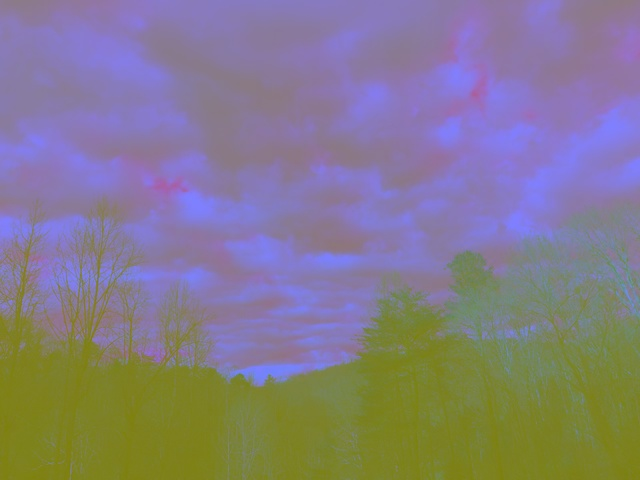
\includegraphics[width=4.5in,natwidth=640,natheight=480]{images/threshold/1.jpg}
						\item A TCbCr digital color space separates the pictures intensity from its colors, enabling a histogram equalization on the blue channel. After performing this equalization, the red-green-blue channels are merged back together. This enables a separation of the sky and clouds from the foreground.\\
							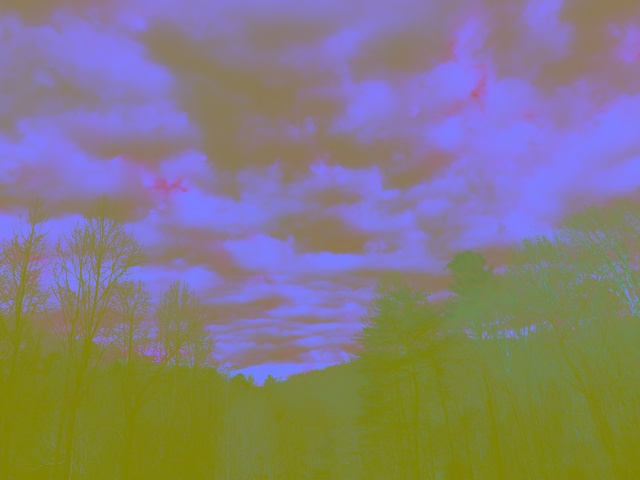
\includegraphics[width=4.5in,natwidth=640,natheight=480]{images/threshold/2.jpg}
						\item This separation of sky and foreground becomes clearer after the image is converted back to BGR.\\
							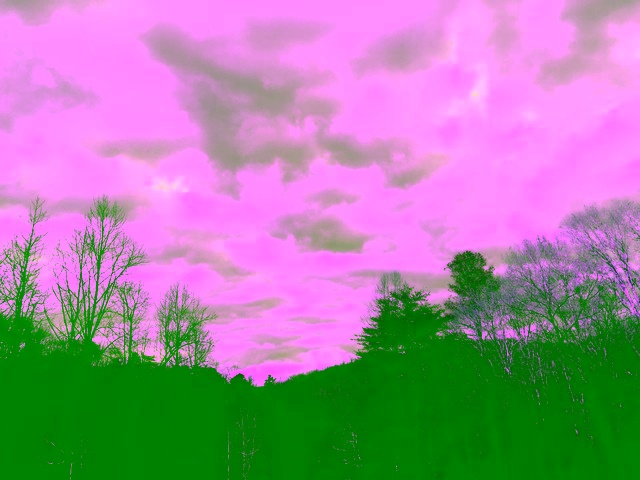
\includegraphics[width=4.5in,natwidth=640,natheight=480]{images/threshold/3.jpg}
						\item Prepare to segment the sky from the foreground by greyscaling the image and applying a gaussian blur.\\
							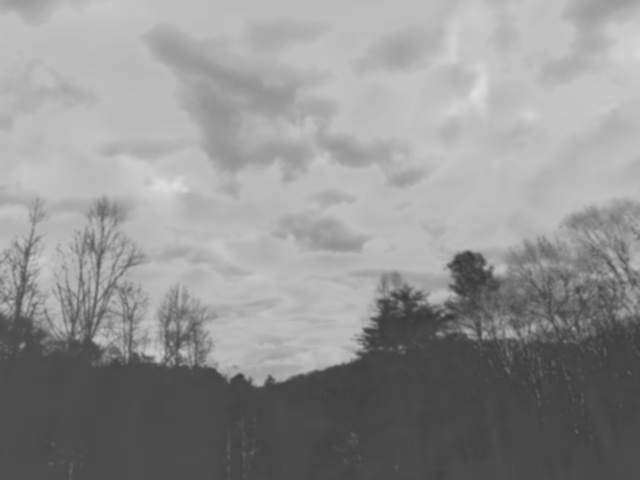
\includegraphics[width=4.5in,natwidth=640,natheight=480]{images/threshold/4.jpg}
						\item Apply a binary threshold; if a pixel value is at least 120, it is assigned grey otherwise it is assigned a black value.\\
							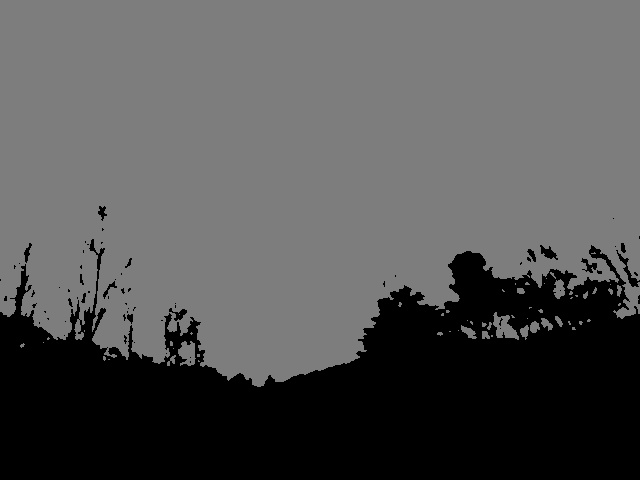
\includegraphics[width=4.5in,natwidth=640,natheight=480]{images/threshold/5.jpg}
						\item Erode the image to de-noise and improve clarity.\\
							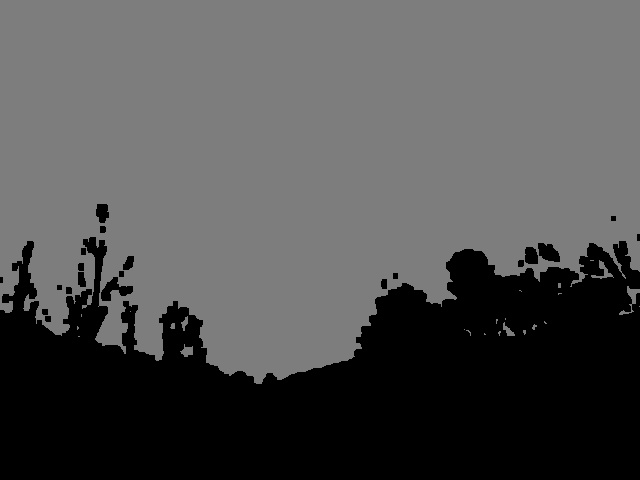
\includegraphics[width=4.5in,natwidth=640,natheight=480]{images/threshold/6.jpg}
						\item Finish de-noise with a dialite to de-chunk the image.\\
							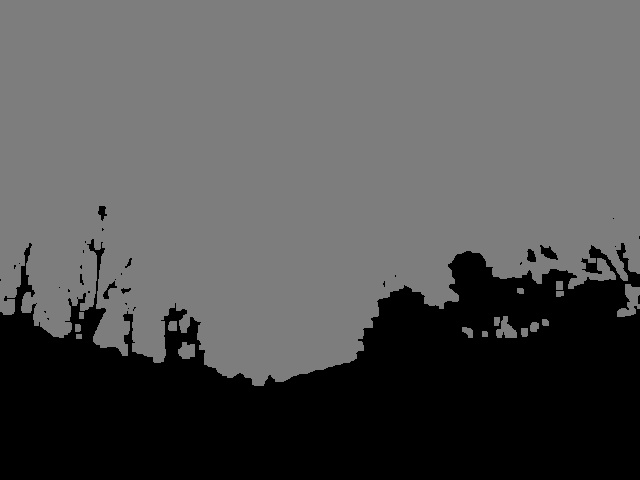
\includegraphics[width=4.5in,natwidth=640,natheight=480]{images/threshold/7.jpg}
						\item Draw contours, in this case it visually appears as a white outline around the largest continuous grey section.\\
							
\includegraphics[width=4.5in,natwidth=640,natheight=480]{images/threshold/8.jpg}
						\item If contours can be drawn, then the largest contour is overlaid on the original image. Fig. Y “passes” as acceptable and as see it accurately outlines the visible sky.\\
							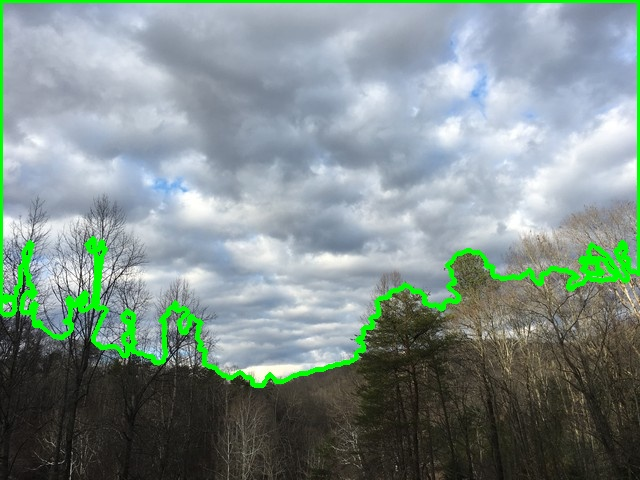
\includegraphics[width=4.5in,natwidth=640,natheight=480]{images/threshold/9.jpg}
						\item If no contours can be drawn, the algorithm fails the image, meaning no sky or horizon can be detected.\\
					\end{enumerate}
					This algorithm struggles to classify low-light images, improvements and fine-tuning are necessary. One can see the threshold algorithm works well for fig. Y.

      \subsubsection{Design Rationale}
      	The Aerolyzer Horizon Detection Filter needs to identify acceptable images, namely ones of the sunset or sunrise. Research indicates that specific sunset or sunrise image classification  necessitates a predictive Tensorflow model because creating such an unsupervised classifier in OpenCV is a challenging task. As demonstrated in Fig. Z, this design rationale is accomplished by incorporating a trained Tensorflow model as a secondary step after OpenCV Horizon Detection by Threshold. Tensorflow analysis is a computationally expensive process. An OpenCV classifier to detect the presence of the sky saves computation time by rejecting all images that do not have skies. If no sky is present then it logically follows that there can be no sunrise or sunset in the image.

      \subsubsection{Design languages}
      	An element in the greater Aerolizer python library, the horizon detection algorithm shall be written in Python 2.7.12 while importing OpenCV 3.3.0 and Numpy 1.13.3. The Aerolyzer project’s sponsor, Dr. Whitehall, chose Python as the library’s primary language. 

\end{singlespace}
\end{document}
